\chapter{Final results and summary discussion}\label{ch:final-results-and-summary-discussion}


\section{Results}\label{sec:results}

Presented model was trained and tested using various parameters.
The changes were affected by the input data as well as the neural network parameters.
The final dataset properties used to train the presented model are described in \mbox{Tab.~\ref{tab:dataset}}.
The input picture size was forced by the used transfer learning model.
This limitation had an effect on resizing original pictures of sequences to the required one by the used neural network.

\begin{table}[!hbt]
    \centering
    \begin{minipage}{.49\textwidth}
        \centering
        \captionsetup{width=\linewidth}
        \captionof{table}{Dataset properties} \label{tab:dataset}
        \begin{tabular}{p{0.6\textwidth}p{0.29\textwidth}}
            \hline
            Human users              & 45                 \\ \hline
            Bot users                & 1                  \\ \hline
            Original sequences       & 639                \\ \hline
            Augmented sequences      & 60 000             \\ \hline
            Minimal sequence length  & 50                 \\ \hline
            Model input picture size & 299 x 299 {[}px{]} \\ \hline
        \end{tabular}
    \end{minipage}
    \hfill
    \begin{minipage}{.5\textwidth}
        \centering
        \captionsetup{width=\linewidth}
        \captionof{table}{Confusion matrix values} \label{tab:confusion-matrix}
        \begin{tabular}{p{0.50\textwidth}p{0.12\textwidth}}
            \hline
            False negatives       & 908   \\ \hline
            False positives       & 215   \\ \hline
            True negatives        & 5 794 \\ \hline
            True positives        & 5 083 \\ \hline
            False rejection rate  & 15.6\% \\ \hline
            False acceptance rate & 3.58\% \\ \hline
        \end{tabular}
    \end{minipage}
\end{table}

The total amount of sequences depends on the minimal sequence length, because sequences that were shorter than 50 were simply rejected.
The sequence split point was established by the time interval between two consecutive actions and in presented work was fixed to 1 second.
The minimal sequence length was fixed based on several attempts.
Shorter sequences than the determined ones resulted in apparently lower accuracy, when longer ones did not improve performance at all.
The length of 50 seemed to be the golden mean between accuracy and amount of sequences.

The charts presented in \mbox{Fig.~\ref{fig:accuracy} and Fig.~\ref{fig:loss}} show that the model accuracy reaches the level of 90\% with 55\% value of the loss function.
It can be seen that the model accuracy during the testing part is in later epochs lower than the one in the training phase.
The difference tends to increase along with the epochs, which is probably caused by the amount of input data.
The impact of the small dataset is also seen on the loss function chart \mbox{(Fig.~\ref{fig:loss})}, where values in the training phase tend to move away from the testing phase ones.

\begin{figure}[!hbt]
    \centering
    \begin{minipage}{.5\textwidth}
        \centering
        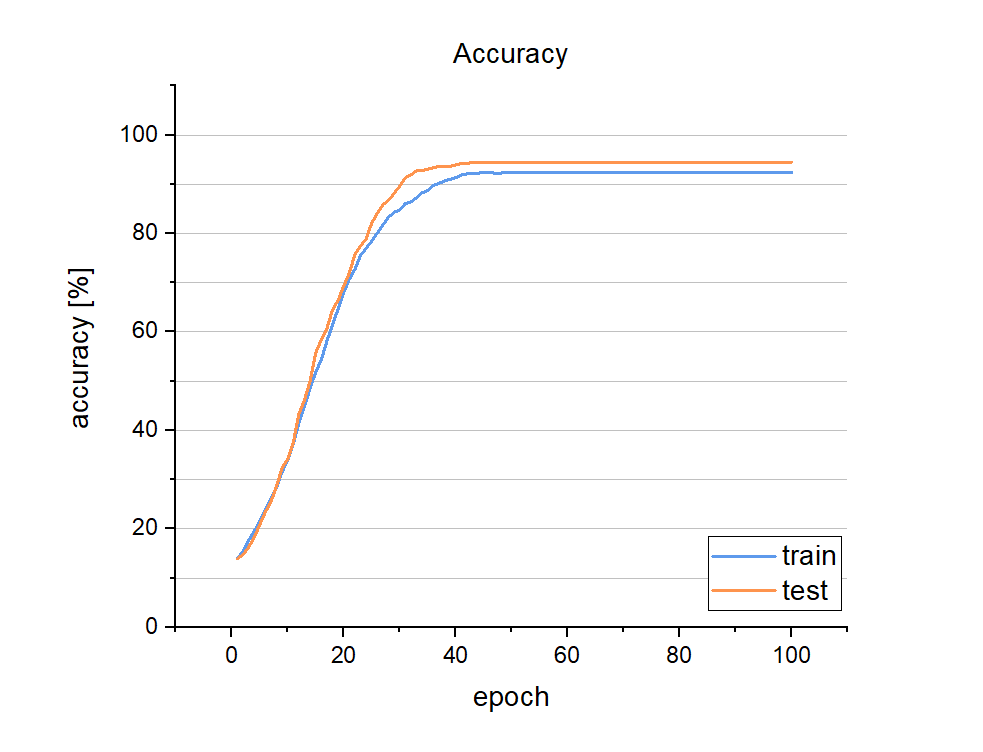
\includegraphics[width=\linewidth]{resources/accuracy.png}
        \captionsetup{width=\linewidth}
        \captionof{figure}{Accuracy of presented model}
        \label{fig:accuracy}
    \end{minipage}%
    \begin{minipage}{.5\textwidth}
        \centering
        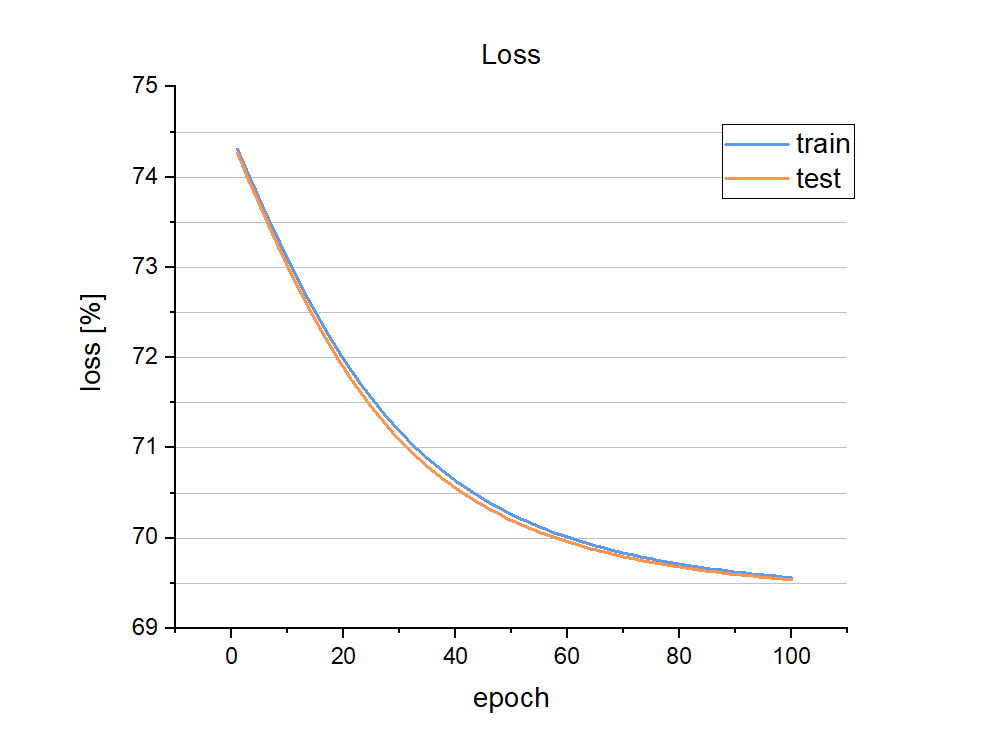
\includegraphics[width=\linewidth]{resources/loss.png}
        \captionsetup{width=\linewidth}
        \captionof{figure}{Value of loss function used in model}
        \label{fig:loss}
    \end{minipage}
\end{figure}

The results presented in \mbox{Tab.~\ref{tab:confusion-matrix}} show that the model has correct prediction, most of the samples are classified to an appropriate category.
The value of \gls{far} is relatively acceptable, however the \gls{frr} is significantly higher than in commercial applications.

Chong et al.~\cite{Main} present similar approach to related problem and in many cases from cited work, authors achieved very low values of \gls{frr} and \gls{far}.
In this work, using \gls{cnn}'s as a core of a solution, a little bit poorer results were achieved.
The authors of this study consider the small dataset as the main foundation of this behavior and despite the data augmentation and other applied techniques, the results did not reach the values from the cited work.

\section{Limitations, conditions and problems}\label{sec:limitations-conditions-problems}
Although the model was considered using different sets of parameters and various approaches, it did not perform as great as was expected.
Due to certain limitations, some aspects of the model performance could not have been improved.
Some problems that have a great impact on the overall results are described in the following sections.

\subsection{Dataset limitation}\label{subsec:dataset-limitation}
The main reason for this performance has to be a small dataset used in the study.
The search for proper and publicly available data resulted in failure.
In other related works, like Chong et al.~\cite{Main} or Antal et al.~\cite{antal2019intrusion} points at the Balabit Mouse Challenge Dataset as the most popular and comprehensive, yet still quite small data source for mouse sequences and behaviors.
However, this dataset is not appropriate for the problem considered in this study.

The Balabit dataset consists of user sessions recorded on the remote machine.
The data includes the timing and position of the mouse cursor of ten different users.
The split dataset represents training sessions and test sessions.
In the training sessions, one can find 65 legitimate sessions of various lengths, wherein total gives 2,253,871 rows of registered user mouse actions.
The test sessions consist of 1,611 shorter sequences, that in total have 2,357,714 recorded actions, where during the session execution of the legal user, the illegitimate action happens --- the session is taken over by another user.
Illegal sessions are the mix of two legitimate users, and when the model considers the example it should assume one user, that is then interrupted and replaced by another user somewhere between the session.

This data does not relate to the problem given in the scope of this work --- the model that can distinguish legitimate human user and non-human bot behavior is taken into consideration.
This particular case is derived from the general problem of distinguishing two or more users and represents a more specific case of using mouse behavioral biometrics.

\subsection{Custom dataset research participation limitation}\label{subsec:custom-dataset-research}
Since no public dataset is available, the goal of this work was to collect exclusive and dedicated data for purpose of the study.
The custom environment\upperref{itm:data-collection} created as a playground for research participants was designed to collect and record the mouse data, but it did not serve the responsiveness of a real commercial website, and therefore it may be causing some confusion among the subject users.
By that means, data collecting was in some kind suggestive and task-oriented.
Given factors could have a negative impact on the quality of the collected data.

The other thing is that participation in the study was completely voluntary and community-based.
The advertisement for the ongoing study was posted on a couple of Facebook groups, which was the most available and large user community base.
However, such an approach resulted in non-supervised data gathering, and therefore some user actions could not be assessed as properly executed and caused disturbances and noises in the set.
The research gathered 63 unique users.
Overall user mouse actions collected are equal to 334,184 rows.
The number of bot actions registered and collected is equal to only 24,791 rows.
Such an uneven ratio of the data made the original dataset imbalanced, which at the beginning resulted in the model making assumptions about every sequence biased towards the class of human users and after data augmentation, the results were significantly better, but not enough to use the solution on the commercial market.

\subsection{Finance limitation}\label{subsec:finance-limitation}
Another problem encountered when preparing the thesis was the limit of the finance intended.\\
Because the research was planned to reach many different users it had to be deployed and hosted on trusted and reliable resources.

Cloud services are really convenient way to handle such a project --- the hosting, computation, and storage resources can be acquired on-demand, with no time and commitment.
In the variety of different cloud solutions, in this case, the Google Cloud Platform was selected and used.
However, the cost of this kind of resources is high enough to be a limitation for the work.

\subsection{Time limitation}\label{subsec:time-limitation}
Due to the time limitation, the duration of the period when the data was collected could not be extended to broader terms, thus the research and the voluntary participation in data collection were canceled during the further implementation of the project --- the bot detection part\upperref{itm:bot-detection}, where the machine learning model was in build.

\section{Conclusions and further study}\label{sec:conclusions-and-further-study}

\subsection{Summary}\label{subsec:summary}
During the work on the presented solution, the steps to limit the impact of the original imbalanced dataset were taken.
Many of them resulted in slightly improved performance or did not improve it at all.
The key factor was the data augmentation, which resulted in a significant increase in the number of samples and also in a better performance.
This technique allowed to convert the unilaterally behaving model into the one whose results are promising for further research.
The linear interpolation, proposed at the beginning, was also very helpful for the model because the additional data was provided to the input which resulted in more close data domain to the ImageNet dataset.
The final results suggest that the augmented dataset admittedly improves and makes the solution promising, but the tendency of moving the training curve away from the testing one should be reviewed.
The authors find the small number of samples as a potential cause of these disturbances, but also the quality of the dataset should be verified.

The presented results verify the data gathering system as a potential source of data for mouse dynamics biometrics researches.
The system is created in a way that it can be easily deployed and tuned to the exact domain requirements.
By using the Kubernetes, it is also scalable and can be even extended to the usage in related problems.
The variety of collected mouse events enables the potential of the system application as a data source for recursive neural networks and also makes it possible to include other events like clicks or scroll actions into the input dataset.

The developed human impersonating bot was created mainly for verification purposes.
The idea of implementation is very simple, but it can be an inspiration for more sophisticated implementations.
The bot as is, can be also used in different problems --- not related to behavioral biometrics.
The possibility of recording the sequences allows for fast and easy configuration which can be important for researches that not focus on the bot implementation but require the bot itself.

The created tools like a serializer/deserializer allows for easily manipulating of the recorded data and transferring it into the input dataset.
The tools related to the Prometheus computing cluster significantly facilitated the work with such an infrastructure and can be considered as a motivation for automation of computing and results obtaining in such an environment.

\subsection{Further study}\label{subsec:further-study}
According to the described issues with the machine learning model, the authors find further study mainly in the improvement of the dataset.
Some efforts may be taken to extend the size of the recorded data.
Firstly, recording sequences of a bigger group of users may be proposed as a solution, especially enlarge the bot users to prevent imbalance.
Such a solution should improve the overall performance of the model or at least suggest other problems related to the quality of the dataset.
If the quality of the recorded samples would be inappropriate, the collection module\upperref{itm:data-collection} should be reviewed and improved.
The main object of interest should be the method of gathering the samples.
Delays and synchronization that can disturb the reliability of the data may be considered as a major area of study.

The different approach that may be taken into consideration is another machine learning model.
In the presented solution, the focus was on the two-dimensional convolutional neural network, taking an example from related works like Chong et al.~\cite{Main} and Wei et al.~\cite{a-deep-learning-approach-to-web-bot-detection-using-mouse-behavioral-biometrics}.
The work~\cite{Main} also shows other solutions, especially recursive neural networks.
Those kinds of neural networks are very popular in problems where the order and time intervals between samples have natural interpretations.
The problem which is described in this work also has similar properties.

These two described areas of study are found by the authors as the major to improve performance and reliability.
To deliver a safe and reliable solution to the commercial market further study is necessary.
